\section{Softwarová část}

\subsection{Nástěnný snímač prostorové teploty}
Programování nástěnných snímačů prostorové teploty jsem využil Arduino IDE, respektive zápis ve Wiring a C++. Zjednodušené blokové schéma programu je na obrázku \ref{fig:blokove-schema-nastenny-snimac-prostorove-teploty-ethernet}. Zařízení neustále kontroluje, zda je připojen do sítě (zda je připojen kabel nebo je k dispozici WiFi síť), pokud zjistí, že není snaží se připojení obnovit. Uživateli je stav připojení signalizován ikonou v levém rohu (zelená barva ikony pro úspěšný stav připojení, červená barva signalizuje problém s připojenín ). Dále zařízení kontroluje připojení k MQTT brokeru (Mosquitto broker), obdobně jako u síťového připojení zařízení se snaží obnovovat automaticky připojení, pokud došlo k výpadku. Stav je opět signalizován pomocí ikony v~levém rohu. Na displeji je červeným písmem zobrazena aktuální naměřená teplota (každých 30 sekund se měří), zeleným písmem je zobrazena požadovaná teplota. Uživatel pravým tlačítek má možnost inkrementovat teplotu o~+0,5 °C, levé tlačítko dekrementuje o -0,5 °C. Střední tlačítko zatím nemá implementovanou funkci. Plánuje se pro vyvolání menu pro další možnosti nastavení (např. pro nastavení hystereze). Poslední řádek s bílým písmem slouží pro zobrazení zprávy uživateli, v současné době je zobrazováno upozornění, zda je potřeba zatopit v krbu. Výše popsáné jednotlivé části jsou vidět na obrázku \ref{fig:software-hanastenny-snimac-prostorove-teploty-zapnuty-displej}. Kód pro nástěnný snímač prostorové teploty je příloze \ref{app:obsah-cd}.

\begin{figure}[H]
    \centering
    \def\svgwidth{\columnwidth}
    \input{images/svg/software/blokove-schema-nastenny-snimac-prostorove-teploty-ethernet.pdf_tex}
    \caption{Blokové schéma softwaru pro nástěnný snímač prostorové teploty.}
    \label{fig:blokove-schema-nastenny-snimac-prostorove-teploty-ethernet}
\end{figure}

\begin{figure}[H]
\centering
\begin{tikzpicture}[font=\sffamily]
     \node[anchor=south west,inner sep=0] (image) at (0,0) {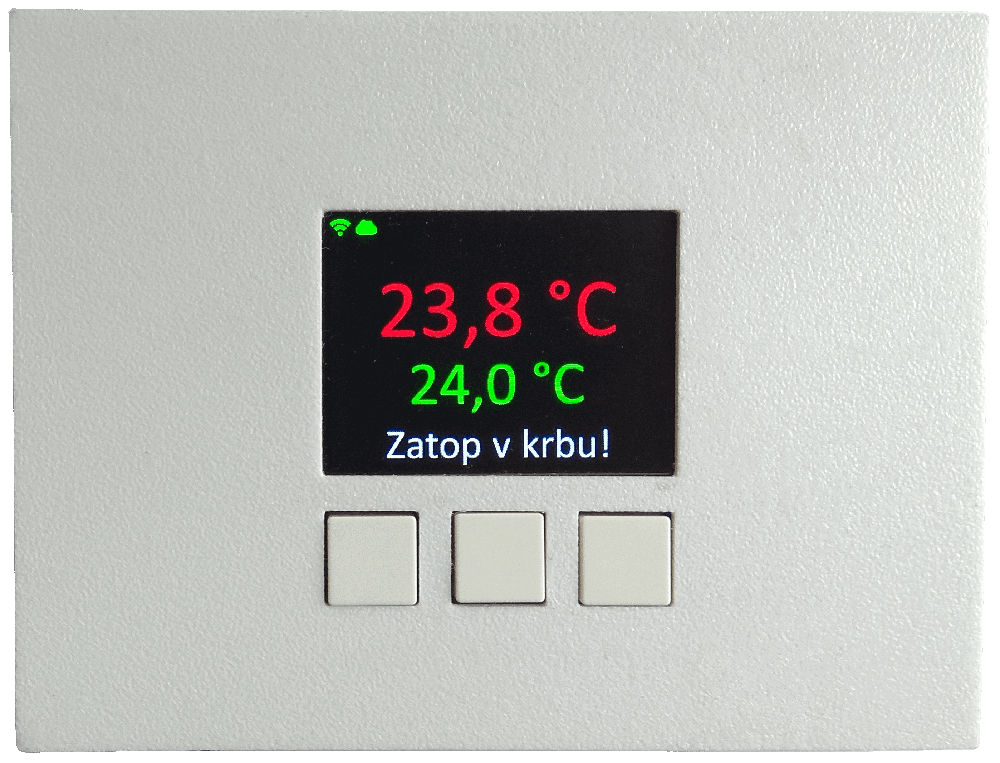
\includegraphics[width=0.9\textwidth]{images/software-ha/nastenny-snimac-prostorove-teploty-zapnuty-displej.png}};
      \begin{scope}[x={(image.south east)},y={(image.north west)}]
     
     %   \draw[help lines,xstep=.1,ystep=.1] (0,0) grid (1,1);
    %    \foreach \x in {0,1,...,9} { \node [anchor=north] at (\x/10,0) {0.\x}; }
       % \foreach \y in {0,1,...,9} { \node [anchor=east] at (0,\y/10) {0.\y}; }
        
          \draw [red,-{Stealth[slant=0]}] (0.2,0.8)--(0.32,0.72);           
          \node[text=red] at (0.2,0.83) {Síťové připojení};
          
          \draw [red,{Stealth[slant=0]}-] (0.38,0.72)--(0.5,0.8);           
          \node[text=red] at (0.5,0.83) {Připojení k MQTT};
          
          \draw [red,-{Stealth[slant=0]}] (0.25,0.6)--(0.37,0.6);
          \node[text=red] at (0.12,0.6) {Aktuální teplota};
          
          \draw [red,{Stealth[slant=0]}-] (0.6,0.5)--(0.72,0.5);
          \node[text=red] at (0.9,0.5) {Požadovaná teplota};
          
          \draw [red,-{Stealth[slant=0]}] (0.25,0.42)--(0.37,0.42);
          \node[text=red] at (0.12,0.42) {Zpráva uživateli};
          
          \draw [red,-{Stealth[slant=0]}] (0.25,0.26)--(0.37,0.26);
          \node[text=red] at (0.1,0.28) {Dekrementování};
          \node[text=red] at (0.1,0.23) {požadované teploty};
          
          \draw [red,{Stealth[slant=0]}-] (0.62,0.26)--(0.74,0.26);
          \node[text=red] at (0.9,0.28) {Inkrementování};
          \node[text=red] at (0.9,0.23) {požadované teploty};
          
          \draw [red,{Stealth[slant=0]}-] (0.5,0.26)--(0.6,0.1);
          \node[text=red] at (0.65,0.1) {Menu};
        \end{scope}
\end{tikzpicture}
\caption{Nástěnný snímač prostorové teploty s informacemi na displeji.}
\label{fig:software-hanastenny-snimac-prostorove-teploty-zapnuty-displej}
\end{figure}

Nastavené QOS pro MQTT přenos zpráv mez WiFi a centrální jednotkou je 2, mezi Ethernetem nástěnným snímač prostorové teploty a centrální jednotkou je 1. Vzhledem k obsahu zpráv, tedy přenosu především naměřené teploty v 30 sekundovém intervalu, by stačilo QOS 0 (především u kabelového připojení). Zároveň pokud dojde přenastavení teploty v centrálním systému, daná změna se projeví i na příslušném nástěnném snímači prostorové teploty. Všechny zařízení mají staticky nastavené IP adresy. Software pro WiFi a Ethernet nástěnný snímač prostorové teploty se liší jen v síťové části. Verze ESP-32-WROVER-IE (M213EH2864UH3Q0) má dvě jádra. V současné verzi není striktně vymezené, které jádro se má používat pro co, dochází k přepínání mezi jádry. Software je udělán s prioritou pro změny uživatele (změna požadované teploty, rozsvícení displeje apod.), tedy aby během změn nedocházelo k prodlevám, které uživatel může registrovat, pokud by se na pozadí něco provádělo (např. odesílání teploty do centrální jednotky, obnova připojení apod.). Pro ověření, že zařízení je připojeno do sítě a komunikuje. Posílá každou minutu aktuální čas do centrální jednotky.


\newpage

\subsection{HA – Typy řízení vytápění}

\label{sec:typy-rizeni-vytapeni}
V rámci řídicího systému existují tyto typy řízení:

\begin{itemize}
  \item Řízení vytápění podle chodbových termostatů.
  \item Řízení vytápění podle nástěnných snímačů prostorové teploty.
  \item Řízení vytápění podle teplotních plánů.
  \item Řízení vytápění podle teplotních plánů s úpravou podle předpovědi počasí.
\end{itemize}

Předpokládá se, že centrální zásobník otopné vody je průběžně ohříván během dne pomocí přebytků energie přes výměníky u krbů. Centrální zásobník otopné vody je dohříván pro případné potřeby vytápění. Je kladena priorita na získávání ohřáté otopné vody ze zdroje tepla zmíněná dříve. Uživatelé jsou upozorňováni signalizací na displejích jak u krbů (obrázek \ref{fig:predni-cast-krytu-vika-instalacni-krabice-krb}), tak i na nástěnných snímačích prostorové teploty (obrázek \ref{fig:software-hanastenny-snimac-prostorove-teploty-zapnuty-displej}), přímo v řídícím systému (možné i upozornění  na mobil (obrázek \ref{fig:mobil-notifikace}), e-mail) či LED diodami (rozsvícení všech) u krbů, že je potřeba zatopit v krbech, pokud systém vyhodnotí, že je potřeb vytápět. V případě, že tomu k tomu nedojde využívá se plynový kondenzační kotel, který dohřívá zásobník otopné vody (ten je možný ovládat automaticky).

\begin{figure}[H]
    \centering
    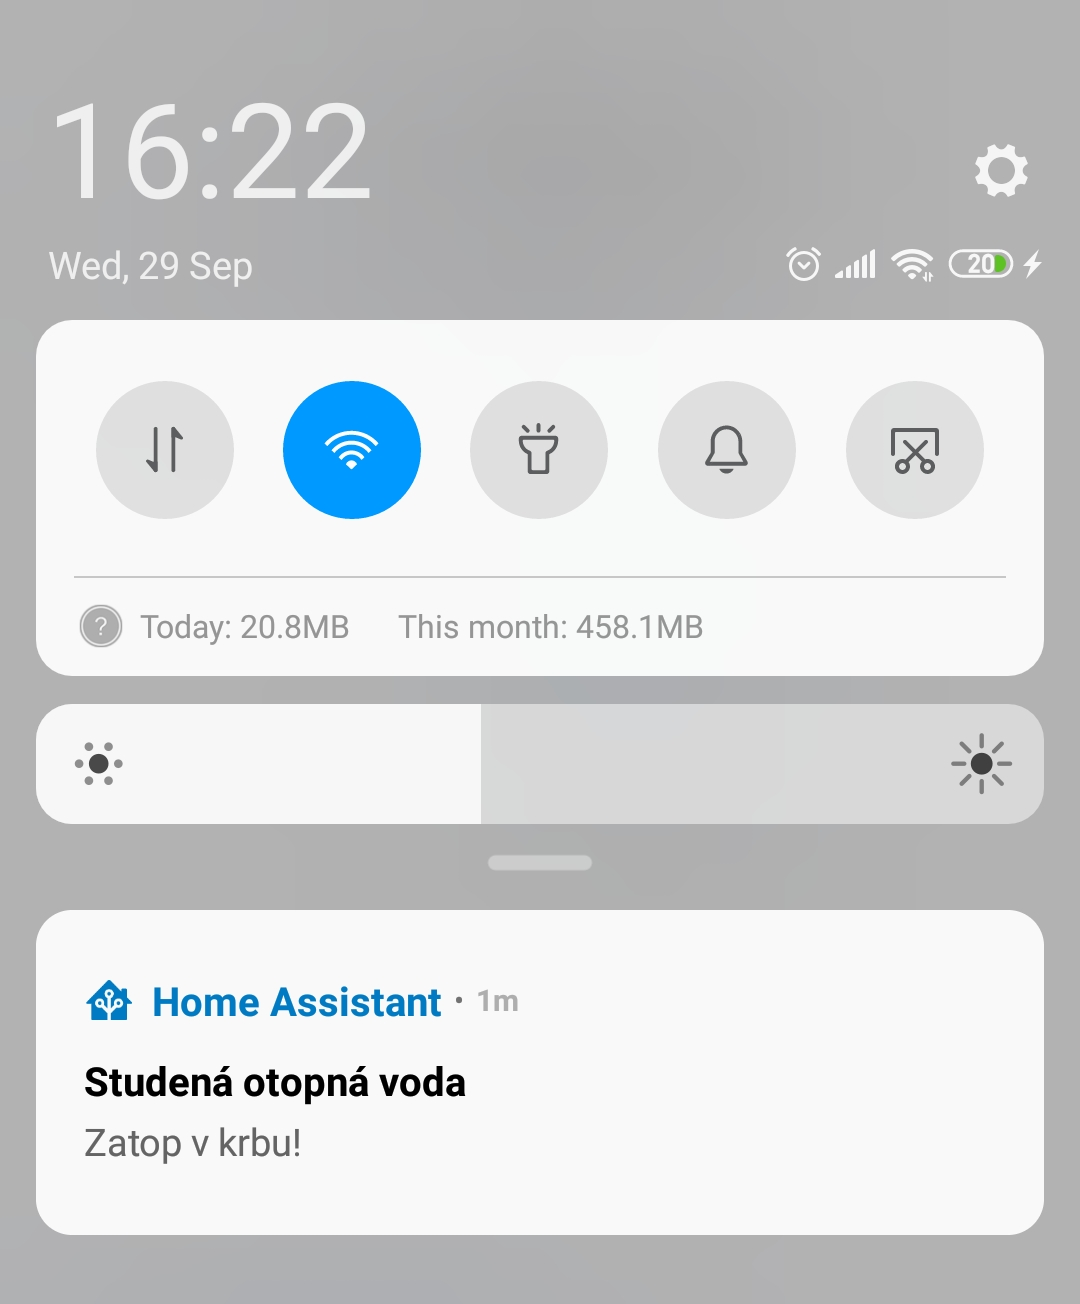
\includegraphics[width=0.4\textwidth]{images/software-ha/mobil-notifikace.png}
    \caption{Upozornění v mobilu.}
    \label{fig:mobil-notifikace}
\end{figure}

Na obrázku \ref{fig:prehled-ha} je rozhraní HA pro nastavení vytápění. V levém menu jsou jednotlivé patra s termostaty a teplotními plány (popsáno níže). V záložce záznamy, historie jsou ukládány do databáze jednotlivé stavy ovládacích prvků a~samotná historie dat, především teplotních senzorů. Dále se zde nachází nastavení uživatelské profilu, tak i celého systému. V horním menu jsou další záložky pro nastavení vytápění, též popsány níže v textu.

\begin{figure}[H]
    \centering
    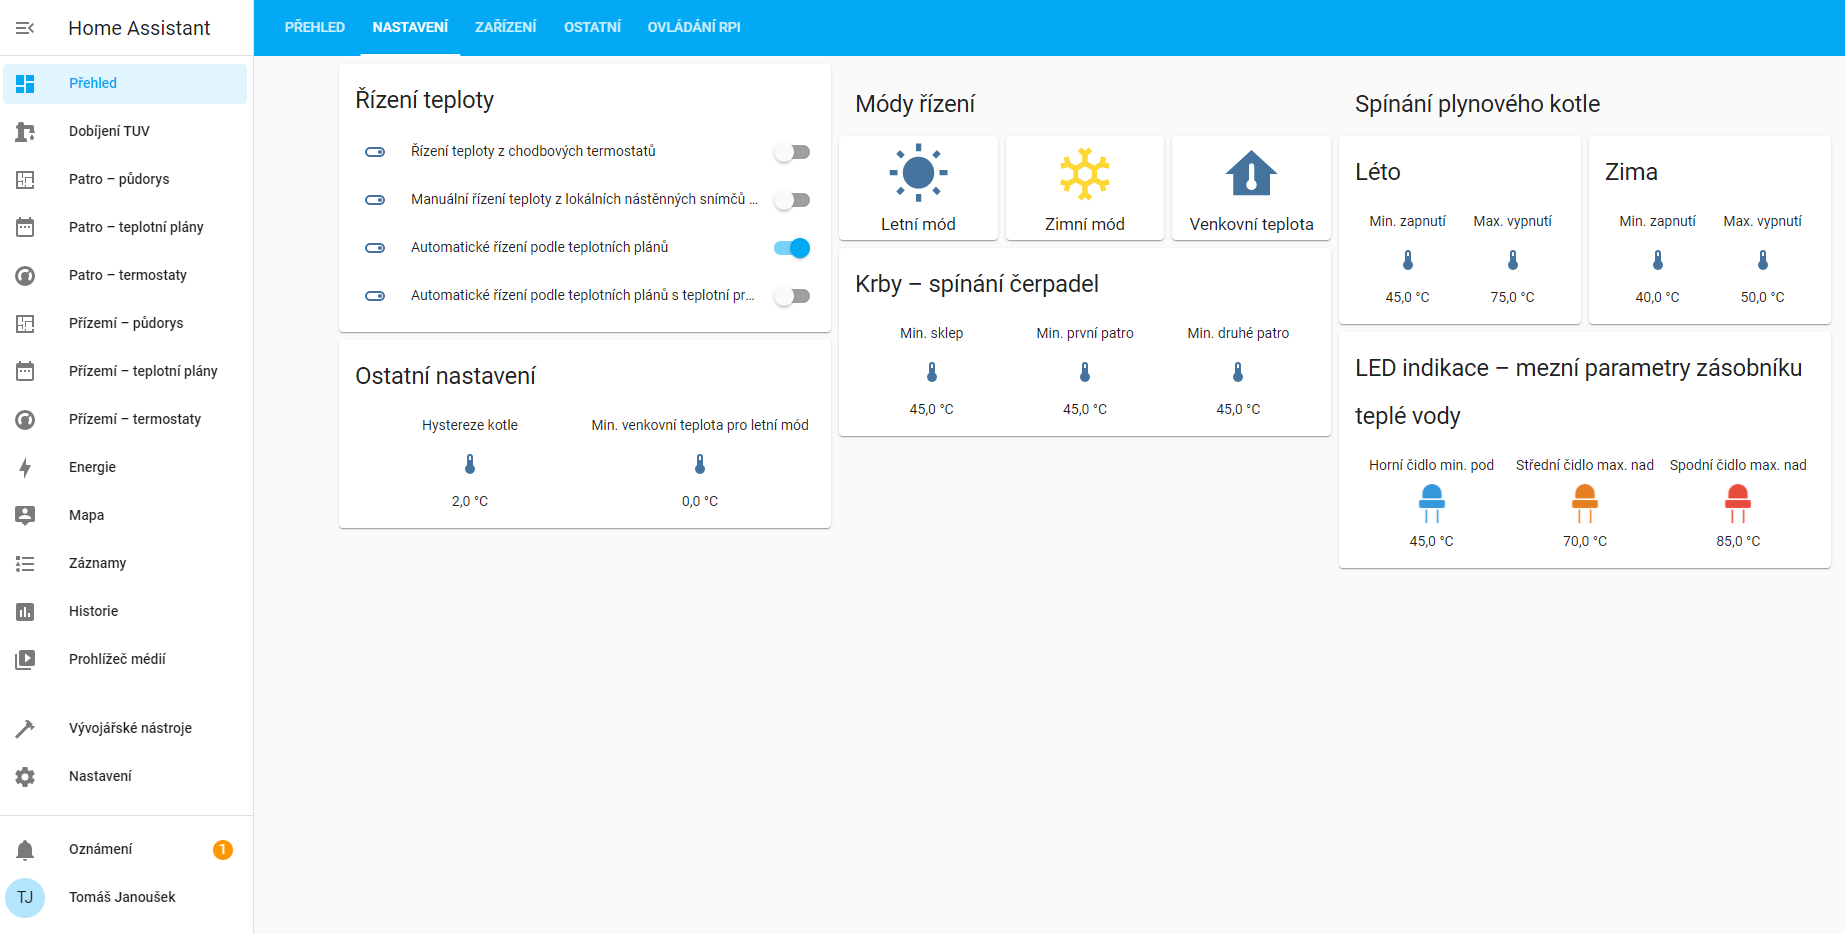
\includegraphics[width=\textwidth]{images/software-ha/prehled-ha.png}
    \caption{Rozhraní HA.}
    \label{fig:prehled-ha}
\end{figure}

V záložce \textbf{přehled} (obrázek \ref{fig:zalozka-prehled}) jsou pro přehlednost zobrazeny aktuální teploty, které se používají pro vyhodnocování v systému HA. V části „jednotlivé teploty“, jsou zde všechny teploty snímané v~zásobníku otopné vody, teploty na kouřovodech v přízemí a patře, v neposlední řadě jez zde i~venkovní teplota. V části „porovnání teploty“ jsou zmíněné teploty zobrazeny v jednom grafu.

\begin{figure}[H]
    \centering
    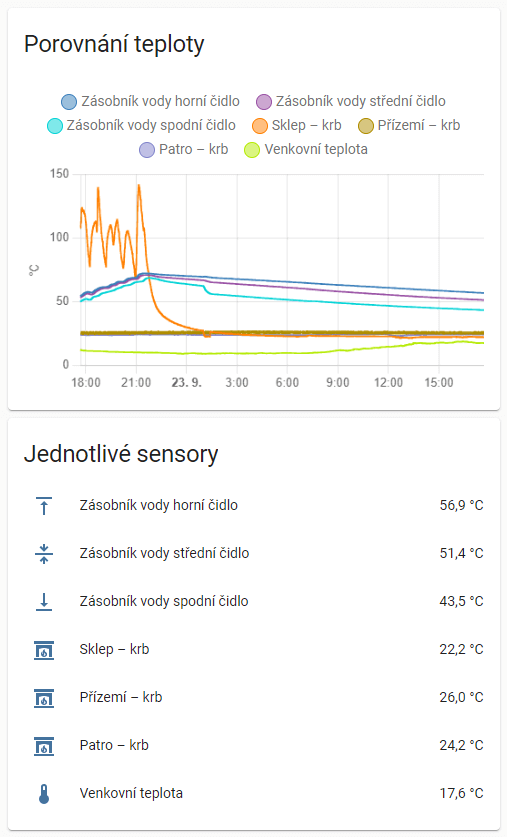
\includegraphics[width=0.6\textwidth]{images/software-ha/zalozka-prehled.png}
    \caption{Záložka přehled v HA.}
    \label{fig:zalozka-prehled}
\end{figure}

V záložce \textbf{nastavení} (obrázek \ref{fig:zalozka-nastaveni}) je možné v části „řízení teploty“ vybrat jeden typ řízení vytápění. Dále v „módy řízení“ je výběr módů a to zimní, letní nebo výběr podle venkovní teploty. Výběr módu má vliv na výběr mezních teplot pro spínání plynového kondenzačního kotle. Dané teplotní meze se dají nastavit v~části „spínání plynového kotle“ (teplotní meze pro léto a zimu). Tyto nastavené meze se berou pro kontrolu s teplotou v horní části zásobníku otopné vody. Pokud teplota v~horní části zásobníku je menší než teplota definovaná v části „min. zapnutí“ dojde k zapnutí kotle pro nahřátí otopné vody, kotel se vypíná při teplota definované v části „max. vypnutí“. Při porovnávání teplot se též bere v potaz nastavená hystereze v~části „ostatní nastavení“. Při výběru módu podle venkovní teploty dochází k~automatickému výběru letního nebo zimního módu. Teplotní mez pro výběr letního módu (v rámci módu podle venkovní teploty) je definovaná v části „min. venkovní teplota pro letní mód“. Toto spínání kotle nastává v momentě, kdy po upozornění uživatelů nedojde k~zatopení v krbech.


V části nastavení „krby – spínání čerpadel“ se definují minimální hranice teploty, kdy dojde k sepnutí oběhových čerpadel pro krbové výměníky, tedy při jaké teplotě se má brát v potaz, zda někdo v krbu zatopit a mají se spustit čerpadla pro nahřívání zásobníku otopné vody. Toto nastavení je poměrně důležité a kontrola těchto teplot je zcela nezávislá na dalších nastaveních (automatizaci) v systému, je potřeba vždy při zatopení spustit čerpadla, jinak dojde k přehřátí vody ve výměníku krbu. V případě přehřátí se aktivuje ochrana přímo u krbů a dojde k ke zvukové signalizaci přehřátí, pokud teplota neklesne za určitou dobu, dojde k aktivování ochranných ventilů a vypuštění přehřáté vody.


V části „LED indikace – mezní parametry zásobníku otopné vody“ se definují mezní teploty pro horní, střední a spodní část zásobníku otopné vody. Tato signalizace se zejména týká pro krby, aby uživatel věděl, zda může topit a jak je moc zásobník nahřátý. U modré LED se definuje mezní minimální teplota, kterou by zásobníku ve horní části měl mít (povolení pro topení). U oranžové LED se definuje mezní maximální teplota, kdy ve střední části zásobníku dochází k dostatečnému nahřátí otopné vody (oznámení, že za chvilku by se mělo přestat topit). U červené LED se definuje mezní maximální teplota, kdy ve spodní části zásobníku je plně ohřátá(okamžitě přestat topit.). Aktivace červené LED předchází v dostatečném předstihu před aktivováním ochrany u~krbů pro přehřátí otopné vody, popsáno v předchozím odstavci.

\begin{figure}[H]
    \centering
    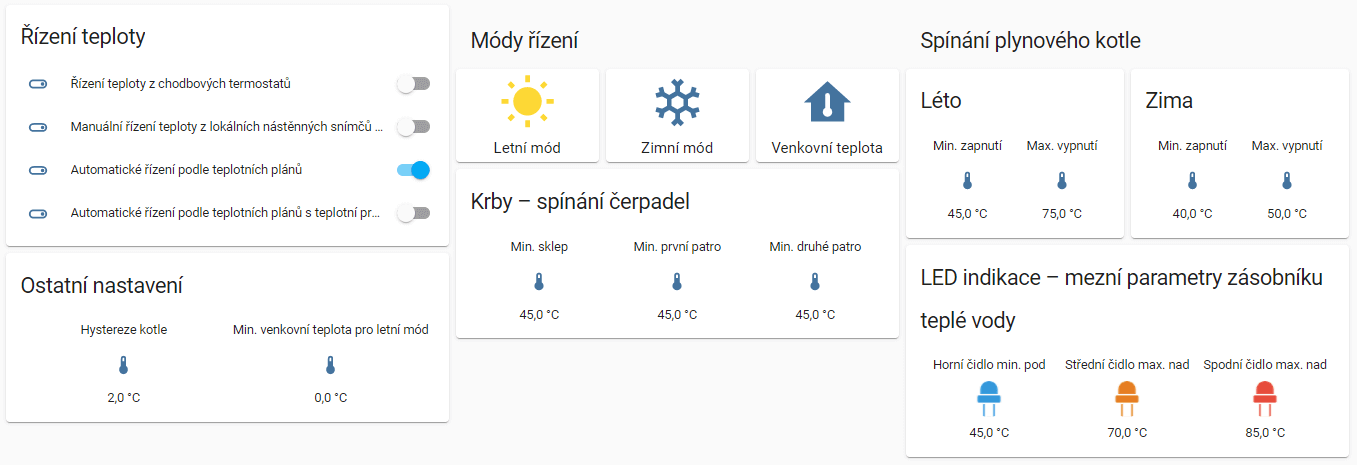
\includegraphics[width=\textwidth]{images/software-ha/zalozka-nastaveni.png}
    \caption{Záložka nastavení v HA.}
    \label{fig:zalozka-nastaveni}
\end{figure}

V záložce \textbf{zařízení} (obrázek \ref{fig:zalozka-zarizeni}) se zobrazují jednotlivá ovládána (zapnuto/vypnuto) zařízení otopné soustavy, tedy plynový kondenzační kotel, čerpadla pro krby s výměníkem, čerpadla pro podlahové vytápění a zapnutí signalizačních LED u krbů. Je možné samotnou automatizaci respektive ovládání zmíněných zařízení řídit podle vlastního uvážení, proto slouží přepínač „manuální ovládání zařízení“, zde si pak uživatel může libovolně jednotlivá zařízení ovládat bez ohledu na nastavenou automatizaci.

V části „termostaty chodby – požadavek topení“, zde se zobrazuje zda dochází k vytápění v přízemí či patře na základě nastavení lokálních termostatů na chodbách.

V části „patro/přízemí – otopné okruhy (ventily)“ se zobrazuje pro přehlednost v procentech úroveň otevření každého ventilu pro daný otopný okruh.

\begin{figure}[H]
    \centering
    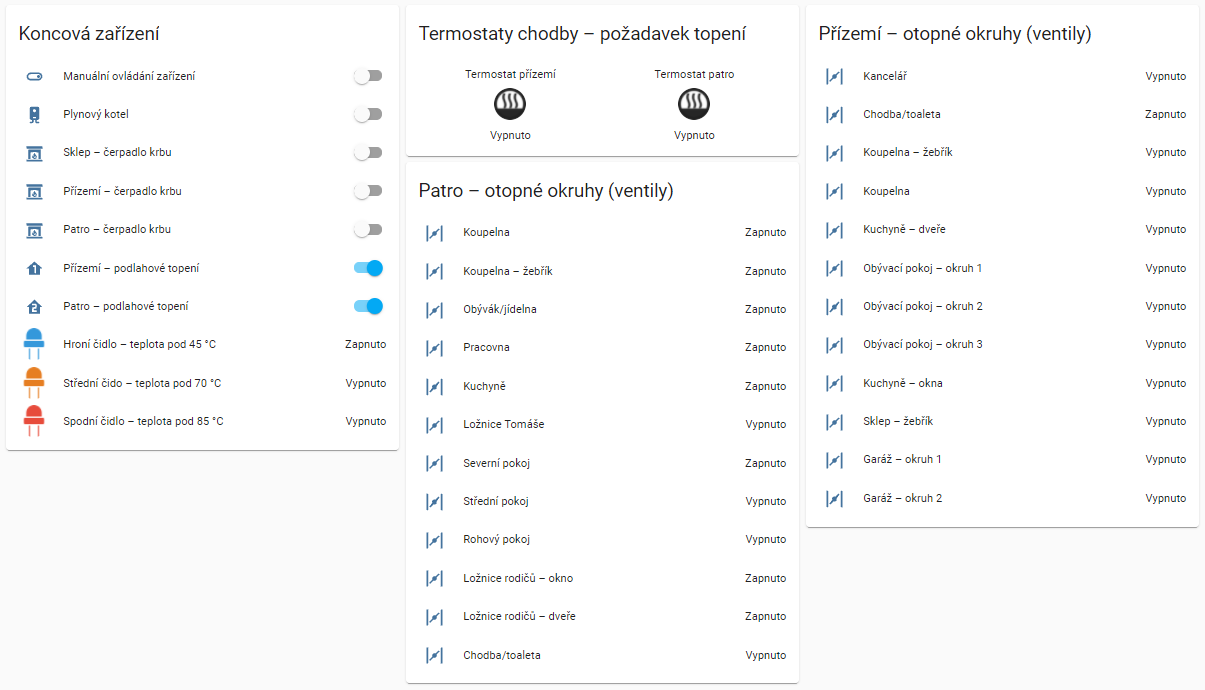
\includegraphics[width=\textwidth]{images/software-ha/zalozka-zarizeni.png}
    \caption{Záložka zařízení v HA.}
    \label{fig:zalozka-zarizeni}
\end{figure}

V záložce \textbf{ostatní} je v části „ovládání čerpadel – vodní kámen“ (obrázek \ref{fig:zalozka-ostatni}) slouží ke spínání čerpadel pro ochranu před zatuhnutím lopatek. Vzhledem k místní dosti tvrdé vodě, došlo při netopení, tedy při nevyužívání daných čerpadel k zatuhnutí lopatek v důsledku nánosu vodního kamene. Pro se zde nachází nastavení, kde si uživatel může pro konkrétní den, hodinu a definovanou délku nastavit spínání čerpadel pro odstranění nánosu na lopatách. Ideální volbou je otopnou vodu zbavit minerálů nebo vyměnit za destilovanou vodu, nicméně k některým méně kvalitnějším provedením spojům trubek otopné soustavy, by docházelo k průsaku otopné vody. Proto je otopná vody z řádu s vyšším podílem minerálů jedním z řešení, jak docílit zaslepení průsaku především vápníkem bez nutnosti, alespoň prozatím, spoje opravovat.

\begin{figure}[H]
    \centering
    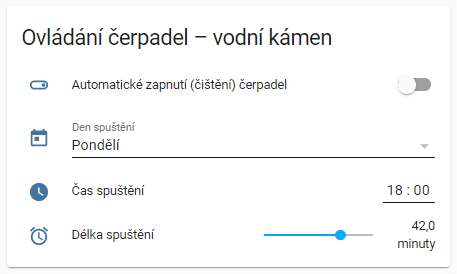
\includegraphics[width=0.7\textwidth]{images/software-ha/zalozka-ostatni.png}
    \caption{Záložka ostatní v HA.}
    \label{fig:zalozka-ostatni}
\end{figure}


\subsubsection{Řízení vytápění podle chodbových termostatů}
V přízemí a v patře je na chodbě umístěn jeden lokání termostat popsaný v~části \ref{sec:digitalni-chodbove-termostaty}. Tento termostat na základě lokálního nastavení (není součástí řídicího systému) spínání/rozpínání výstupní relé při požadavku na vytápění. Tento požadavek se následně vyhodnotí v centrálním systému (popsáno v části \ref{sec:typy-rizeni-vytapeni} v části zařízení) a dojde k sepnutí nebo rozepnutí daného chodbového oběhového čerpadlo pro podlahové vytápění a~otevření všech okruhů podlahové vytápění. Dochází tedy k řízení vytápění všech místností na patře podle jednoho centrálního termostatu. 

\subsubsection{Řízení vytápění podle nástěnných snímačů prostorové teploty}
\label{sec:rizeni-vytapeni-podle-nastennych-snimacu-prostorove-teploty}
Podle aktuální teploty naměřenou z každé místnosti je ovládán daný otopný okruh pro vytápění. Na základě požadované teploty, kterou je možné zadat přímo v systému HA (viz obrázek \ref{fig:lokalni-termostat-ha}) nebo je možné teplotu nastavit přímo v~místnosti pomocí tlačítek na nástěnném snímači prostorové teploty, tím dojde k přenesené požadované teploty do systému a zobrazení na daném termostatu, nastavení funguje i opačně. Řízení vytápění místnosti je dáno hysterezí 0,5~°C. Regulace vytápění tedy reaguje na aktuální naměřenou teplotu.

\begin{figure}[H]
    \centering
    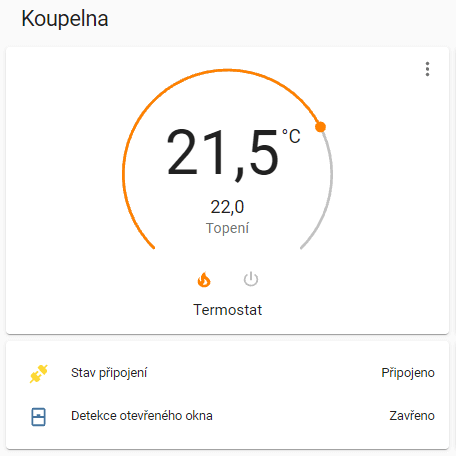
\includegraphics[width=0.6\textwidth]{images/software-ha/lokalni-termostat-ha.png}
    \caption{Nástěnný snímač prostorové teploty v HA.}
    \label{fig:lokalni-termostat-ha}
\end{figure}

Lokální termostaty jsou roztříděny do skupiny podle daného patra, kde se nalezení, tedy termostaty pro přízemí a patro (příklad sdružení termostatů pro patro je na obrázeku \ref{fig:prehled-lokalnich-termostaty-patro}, obdobně vypadá i pro přízemí).

\begin{figure}[H]
    \centering
    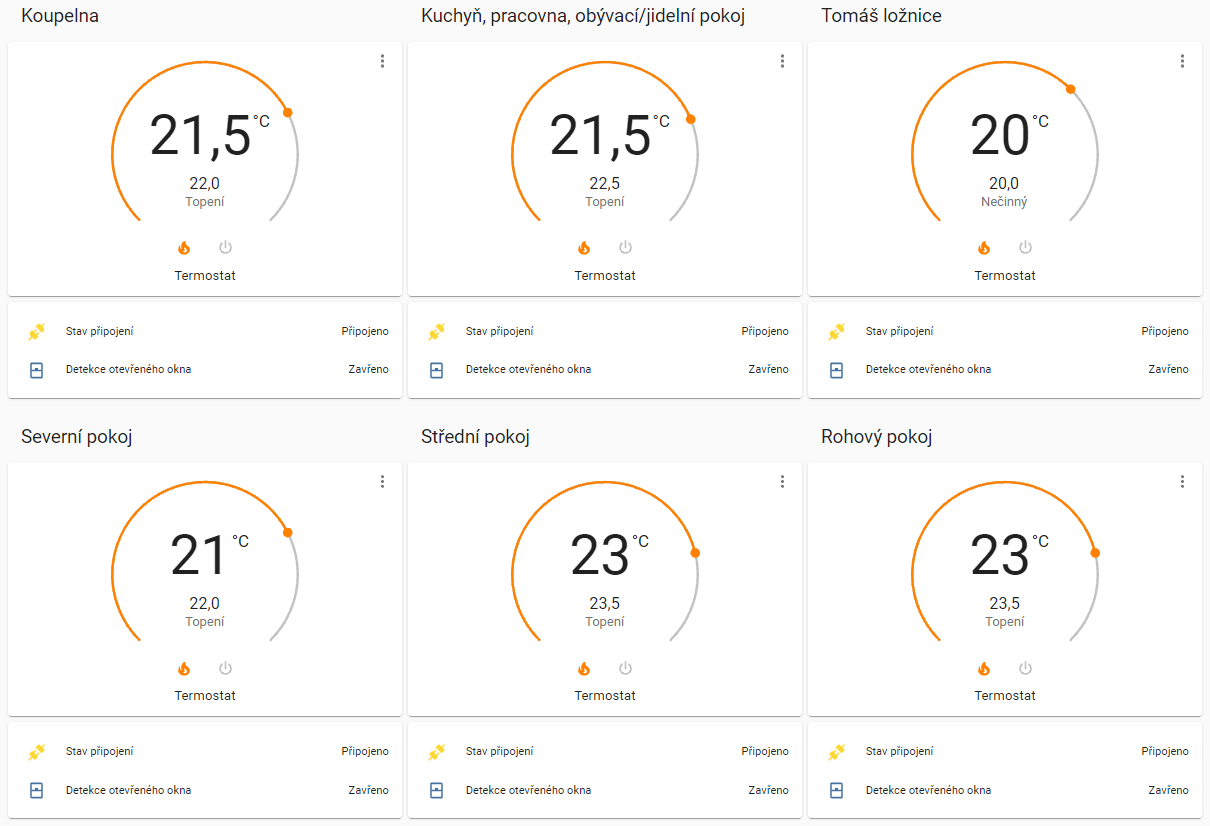
\includegraphics[width=\textwidth]{images/software-ha/prehled-lokalnich-termostaty-patro.png}
    \caption{Výběr nástěnných snímačů prostorové teploty v HA pro patro.}
    \label{fig:prehled-lokalnich-termostaty-patro}
\end{figure}

Každý termostat má dále zobrazení, zda je koncový snímač prostorové teploty připojen k centrální jednotce, ověření probíhá na základě posílaní aktuálního času, který se porovnává s časem v centrální jednotce zpožděný o~minutu, pokud zařízení neposílá aktuální čas, dojde ke zpoždění a zařízení se vyhodnotí jako nepřipojené. Pokud je zařízení nepřipojené, tak dojde k~zastavení vytápění pro danou místnost, dokud není spojení obnoveno. Dále je zde detekce otevřeného okna, tato funkce je více popsána v části \ref{sec:detekce-otevreneho-okna}. V~případě otevřeného okna je uživatel informován pomocí upozornění. 



\subsubsection{Řízení vytápění podle teplotních plánů} 
\label{sec:rizeni-vytapeni-podle-teplotnich-planu}
Další možností řízení vytápění jednotlivých místností je podle nadefinovaných časových plánů. Uživatel má možnost si pro každou místnost v rámci 24 hodin nadefinovat časové úseky s danou požadovanou teplotou. Takto nastavené časové plány se průběžně kontrolují systémem a nastavuje aktuálně požadovanou teplotu do lokálních nástěnných snímačů teploty, tato teplota se objeví i na termostatu v HA (viz obrázek \ref{fig:lokalni-termostat-ha}). Následně dochází k regulaci vytápění podle popisu v části \ref{sec:rizeni-vytapeni-podle-nastennych-snimacu-prostorove-teploty}. Rozhraní pro nastavení časových úseků je na obrázku \ref{fig:teplotni-plan-ha}. Uživatel si může jednotlivé úseky přidávat nebo odebírat (min. počet časových úseků jsou dva). Uživatel má na výběr zda se časové úseky aplikují na všechny v dny v týdnu nebo jen pracovní dny, víkend či výběr konkrétních dnů v týdnu. Dále je možné nadefinovat, zda se pro daný úsek má vytápět nebo naopak nemá.

\begin{figure}[H]
    \centering
    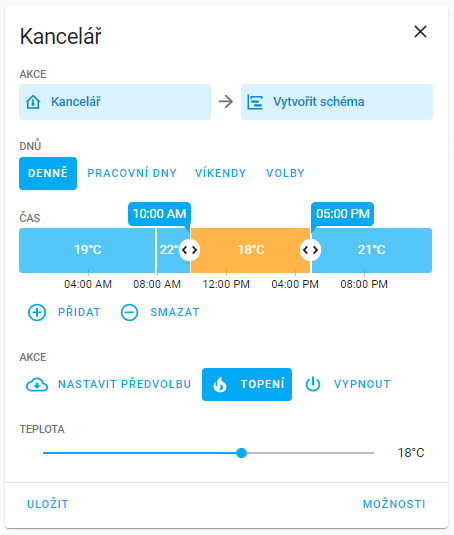
\includegraphics[width=0.8\textwidth]{images/software-ha/teplotni-plan-ha.png}
    \caption{Rozhraní pro nastavení teplotního plánu.}
    \label{fig:teplotni-plan-ha}
\end{figure}

Pro každou místnost je možné nadefinovat libovolný počet časových plánů. Přehled jednotlivých plánů je zobrazen pod každým dnem, viz obrázek \ref{fig:teplotni-plany-ha}. Jednotlivé plány je také možné pozastavit pomocí posuvného tlačítka vpravo. Celkový přehled teplotních plánů všech místností pro patro je vidět na obrázku \ref{fig:teplotni-plany-prehled-ha}, obdobně vypadá i pro přízemí.

\begin{figure}[H]
    \centering
    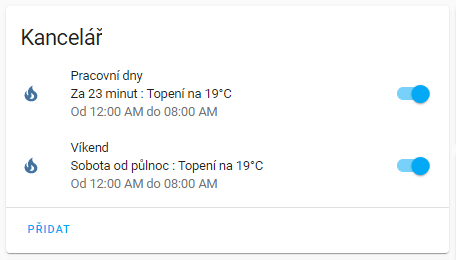
\includegraphics[width=0.7\textwidth]{images/software-ha/teplotni-plany-ha.png}
    \caption{Jednotlivé plány pro danou místnost.}
    \label{fig:teplotni-plany-ha}
\end{figure}


\begin{figure}[H]
    \centering
    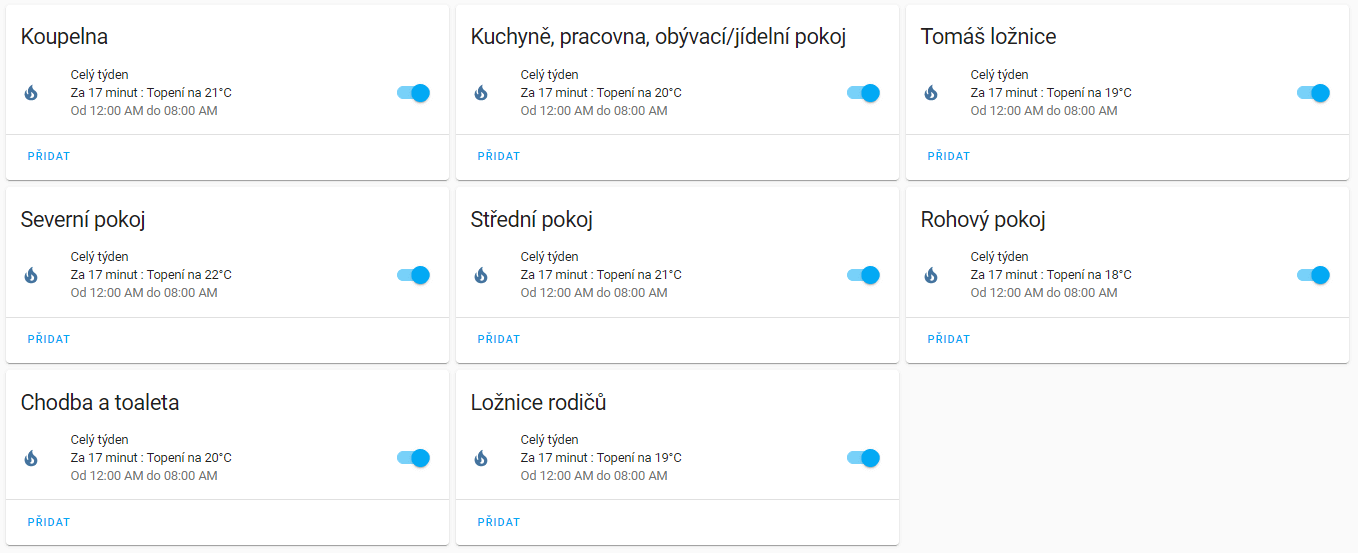
\includegraphics[width=\textwidth]{images/software-ha/teplotni-plany-prehled-ha.png}
    \caption{Přehled teplotních plánů pro patro.}
    \label{fig:teplotni-plany-prehled-ha}
\end{figure}

\subsubsection{Řízení vytápění podle teplotních plánů s úpravou podle předpovědi počasí.} 
\label{sec:rizeni-vytapeni-podle-teplotnich-planu-s-upravou-podle-predpovedi-pocasi}
Řízení vytápění podle teplotních plánů s úpravou podle předpovědi počasí probíhá obdobně, jako v případě popisu v části \ref{sec:rizeni-vytapeni-podle-teplotnich-planu}. Rozdílem je, že jednou týdně si systém „ošahá“ místnost a určí si převodní charakteristiku podle které  upravuje teplotní plány (více v části \ref{sec:teplotni-predikce}).

\subsection{Inteligentní část}
\subsubsection{Detekce otevřeného okna}
\label{sec:detekce-otevreneho-okna}
Pro detekci otevřeného okna se vyhodnocuje gradient teploty. Tato funkce je již v HA integrovaná pomocí platformy Trend, bylo nutné definovat samotný gradient, tedy číslo pro minimální změnu teploty za určité časové období, kdy dojde k detekci otevřeného okna (poklesu teploty v místnosti). Detekce není vždy přesná, optimální je použít samotný senzor pro detekci otevřeného okna (magnetický senzor), nicméně tento senzor je nutné montovat na každé okno (cenové prodražení, nutné další kabely).

\subsubsection{Teplotní predikce}
\label{sec:teplotni-predikce}
Na základě historický dat (7 dní) systém automaticky provádí pro každou místnost zvlášť takzvané „teplotní ošahání místnosti“ spočívající v matematické metodě lineární regrese (aproximace naměřených hodnot metodou nejmenších čtverců). Podle vnitřní, venkovní teploty a doby zapnutí jednotlivých termoelektrických pohonů (doby vytápění) pro danou místnost se získá převodní charakteristika, závislost doby vytápění na rozdílu vnitřní a venkovní teploty. Tato jednoduchá aproximace se využívá pro definované teplotní plány (část \ref{sec:rizeni-vytapeni-podle-teplotnich-planu-s-upravou-podle-predpovedi-pocasi} Řízení vytápění podle teplotních plánů s úpravou podle předpovědi počasí). Z jednotlivých teplotních úseků se vezme jejich začátek a pro danou hodinu se vybere teplota z předpovědi počasí. Tato teplota se následně využívá v dané lineární aproximace a určí se v minutách o kolik je nutné úsek posunout. Tím se zajistí, že v požadovaný čas bude v~místnosti požadovaná teplota. Každý týden se udělá nová lineární aproximace pro danou místnost.


\section{Zápis automatizace}
Primárně pro zápis automatizace se využívá \acrshort{yaml} (\textit{\acrlong{yaml}}). Dále mezivrstvu mezi systémem HA a využití vlastních Python knihoven s návazností na objekty v HA využívám AppDaemon (externí modul). Appdaemon využívám pro obsluhu LCD displejů, zónových regulátorů, teplotních čidel,pro čtení hodnoty z chodbových termostatů a pro předpřípravu dat pro „ošahání teploty v místnosti“.. 

\subsection{Přidání grafických komponent}
Obecně u komponent jsou povinné a nepovinné položky (mají svojí výchozí hodnotu). Mezi ty povinné tedy patří výběr komponenty, kterou chceme (input$\_$text, input$\_$select, input$\_$boolean apod.), dále název komponenty (lze volitelně zvolit) přes který dále s komponentou pracujeme například v~automatizaci. O tom, co je a není povinné se dozvíme v dokumentaci každé komponenty na webu HA.

Příklad přidání komponenty input$\_$text. Input$\_$text nám říká jakou komponentu chceme, dále následuje název této komponenty, přes tento název dále v programu přistupujme k této komponentě. Dále je zde řádek s name,
jedná se o název, který se zobrazí uživateli. Initial je počáteční text, který se zobrazí. Min definuje minimální délku řetězce. Max definuje maximální délku řetězce. Pattern validuje vstup, jaké znaky jsou povoleny.

\begin{lstlisting}
input_text:
	name_input_text:
		name: "Zobrazený název v gui"
		initial: "Inicializační text"
		min: 8
		max: 40
		pattern: "[a-fA-F0-9]*"
\end{lstlisting}

\subsection{Konfigurace automatizace}

Automatizace se skládá ze tří základních částí:

\begin{itemize}
\item Spouštěč automatizace, spuštění může být například, že někdo přijde
domů, je zapnuto tlačítko, zajde Slunce, spouštěč může být konkrétní
čas, datum apod.
\item Podmínka omezující spouštěč. Může se jednat třeba o časovou podmínku, že aktuální čas se musí rovnat požadovanému. Zadaný vstup musí
být větší než požadované číslo apod.
\item Akce vykonaná při splnění všech podmínek. Akcí může být zapnutí
zařízení, zobrazení upozornění, poslání sms apod.
\end{itemize}

Příklad automatizace:

\begin{lstlisting}
(spouštěč) Když Pavel dorazí domů
(podmínka) a Slunce zapadlo
(akce) 	   Rozsviť světla v obývacím pokoji
\end{lstlisting}

%\section{Výměna dat mezi centrální jednotkou a~nástěnnými snímači prostorové teploty}
%Jak již bylo řečeno v části \ref{sec:mqtt-protokol} pro výměnu dat mezi centrální jednotkou a~nástěnnými snímači prostorové teploty využívám MQTT protokol. Nástěnný snímač prostorové teploty posílá do centrální jednotky aktuálně naměřenou teplotu pro danou místnost, případně pokud uživatel změní požadovanou teplotu, tato změna se projeví i v systému. Naopak pokud v systému dojde ke změně požadované teploty, tato teplota se projeví i v  nástěnném snímači prostorové teploty pro danou místnost. Dále pokud je požadavek, aby uživatelé začali topit v krbech (viz část \ref{sec:typy-rizeni-vytapeni}) a nedojde k tomu stavu za určitou dobu, jsou uživatelé informování zprávou na displeji. 

%\section{Síťová část}
%Všechny nástěnné snímače prostorové teploty mají přidělenou statickou IP adresu. Též mají definovanou vlastní MAC adresu. Je možné využít i DHCP, ale pro stálost zařízení jsem využil statické IP adresy. Do rozhraní HA, lze vstoupit přes webový prohlížeč s adresou http:$\slash \slash$homeassistant:8123 nebo http:$\slash \slash$ip$\_$adresa$\_$rpi:8123. Lze pro přístup využít i mobilní telefon s Android nebo iOS systémem, kterou lze oficiálně stáhnout z daných obchodů s~aplikacemi. Celé rozhraní je velmi responzivní, viz obrázek \ref{fig:mobilni-aplikace} pro systém Android.

%\begin{figure}[H]
%    \centering
%    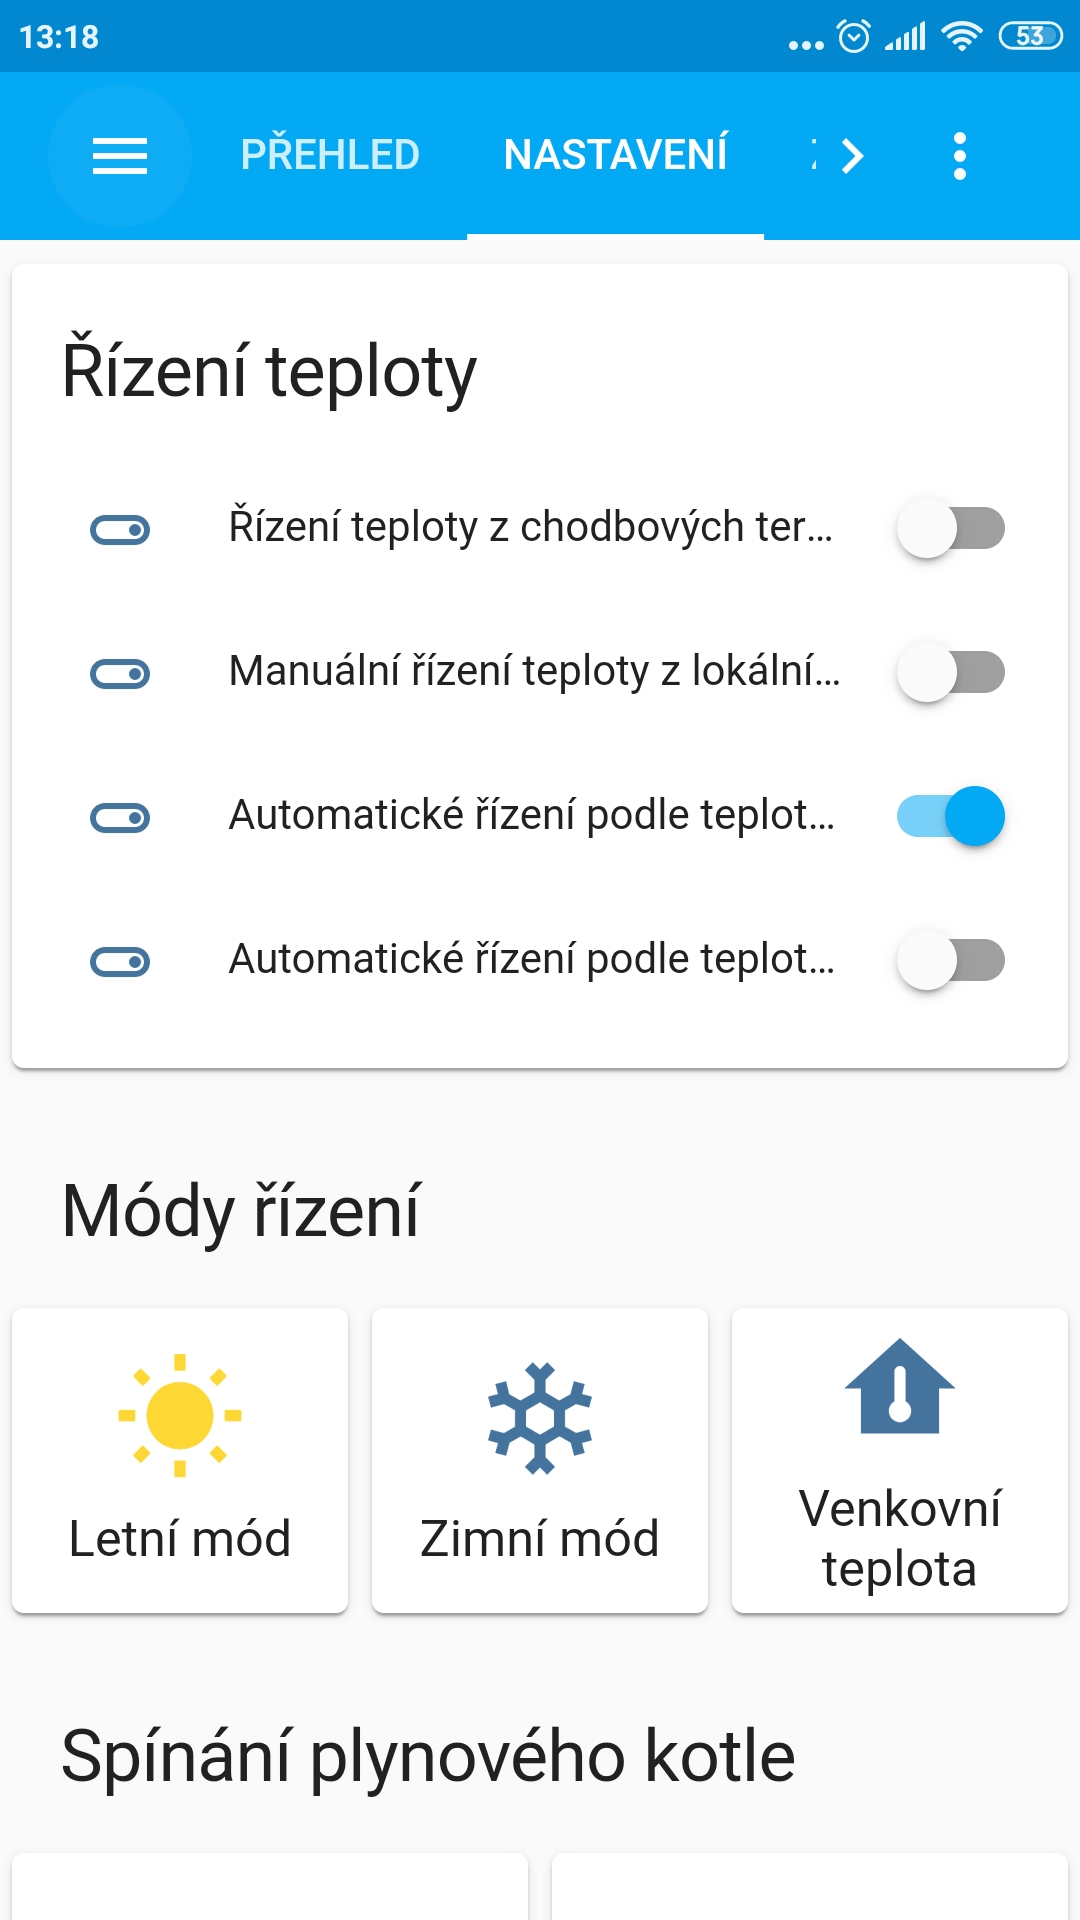
\includegraphics[width=0.8\textwidth]{images/mobilni-aplikace/mobilni-aplikace.png}
%    \caption{Mobilní aplikace na Android.}
%    \label{fig:mobilni-aplikace}
%\end{figure}




